\fancyfoot[C]{G�rel}
\paragraph{Fertigung der Platine}

Die Herstellung von Platinen f�r den Anschluss der Elektronischen Ger�te und Sensoren im Auto ist unvermeidlich. 
Die Verwendung von Platinen bietet zahlreiche Vorteile, da sie eine Vielzahl von Steckverbindungen und Komponenten aufnehmen k�nnen, 
die mit herk�mmlicher Drahtverbindungen technisch nur schwer realisierbar w�ren.

\begin{figure}[H]
    \centering
    \begin{minipage}[b]{0.45\textwidth}
        \centering
        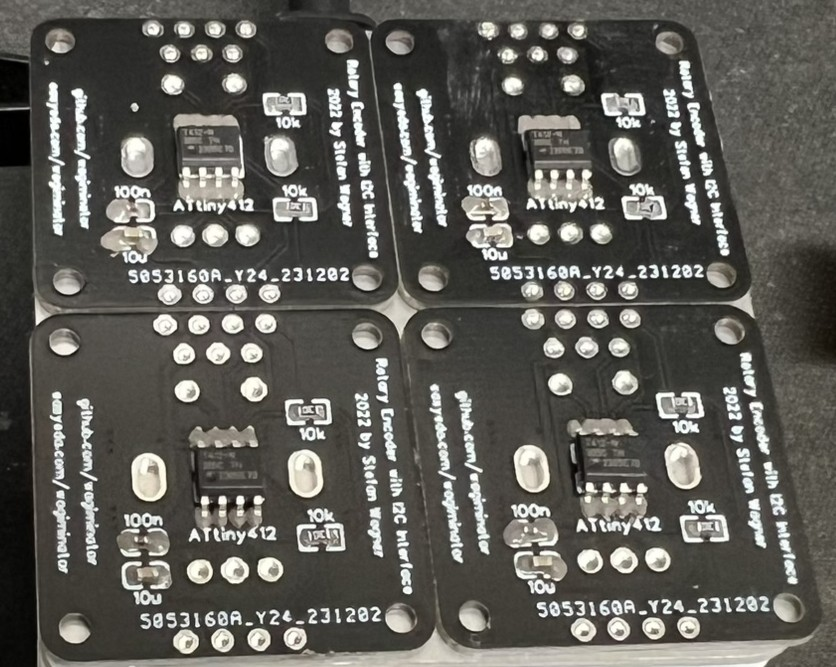
\includegraphics[scale=1]{./3_Stand_der_Technik/Abbildungen/beispiel_bild_anfertigung_reflow.JPEG}
        \caption{Symbolfoto, anfertigung von best�ckten Platinen}
    \end{minipage}
    \hfill
    \begin{minipage}[b]{0.45\textwidth}
        \centering
        \rotatebox{90}{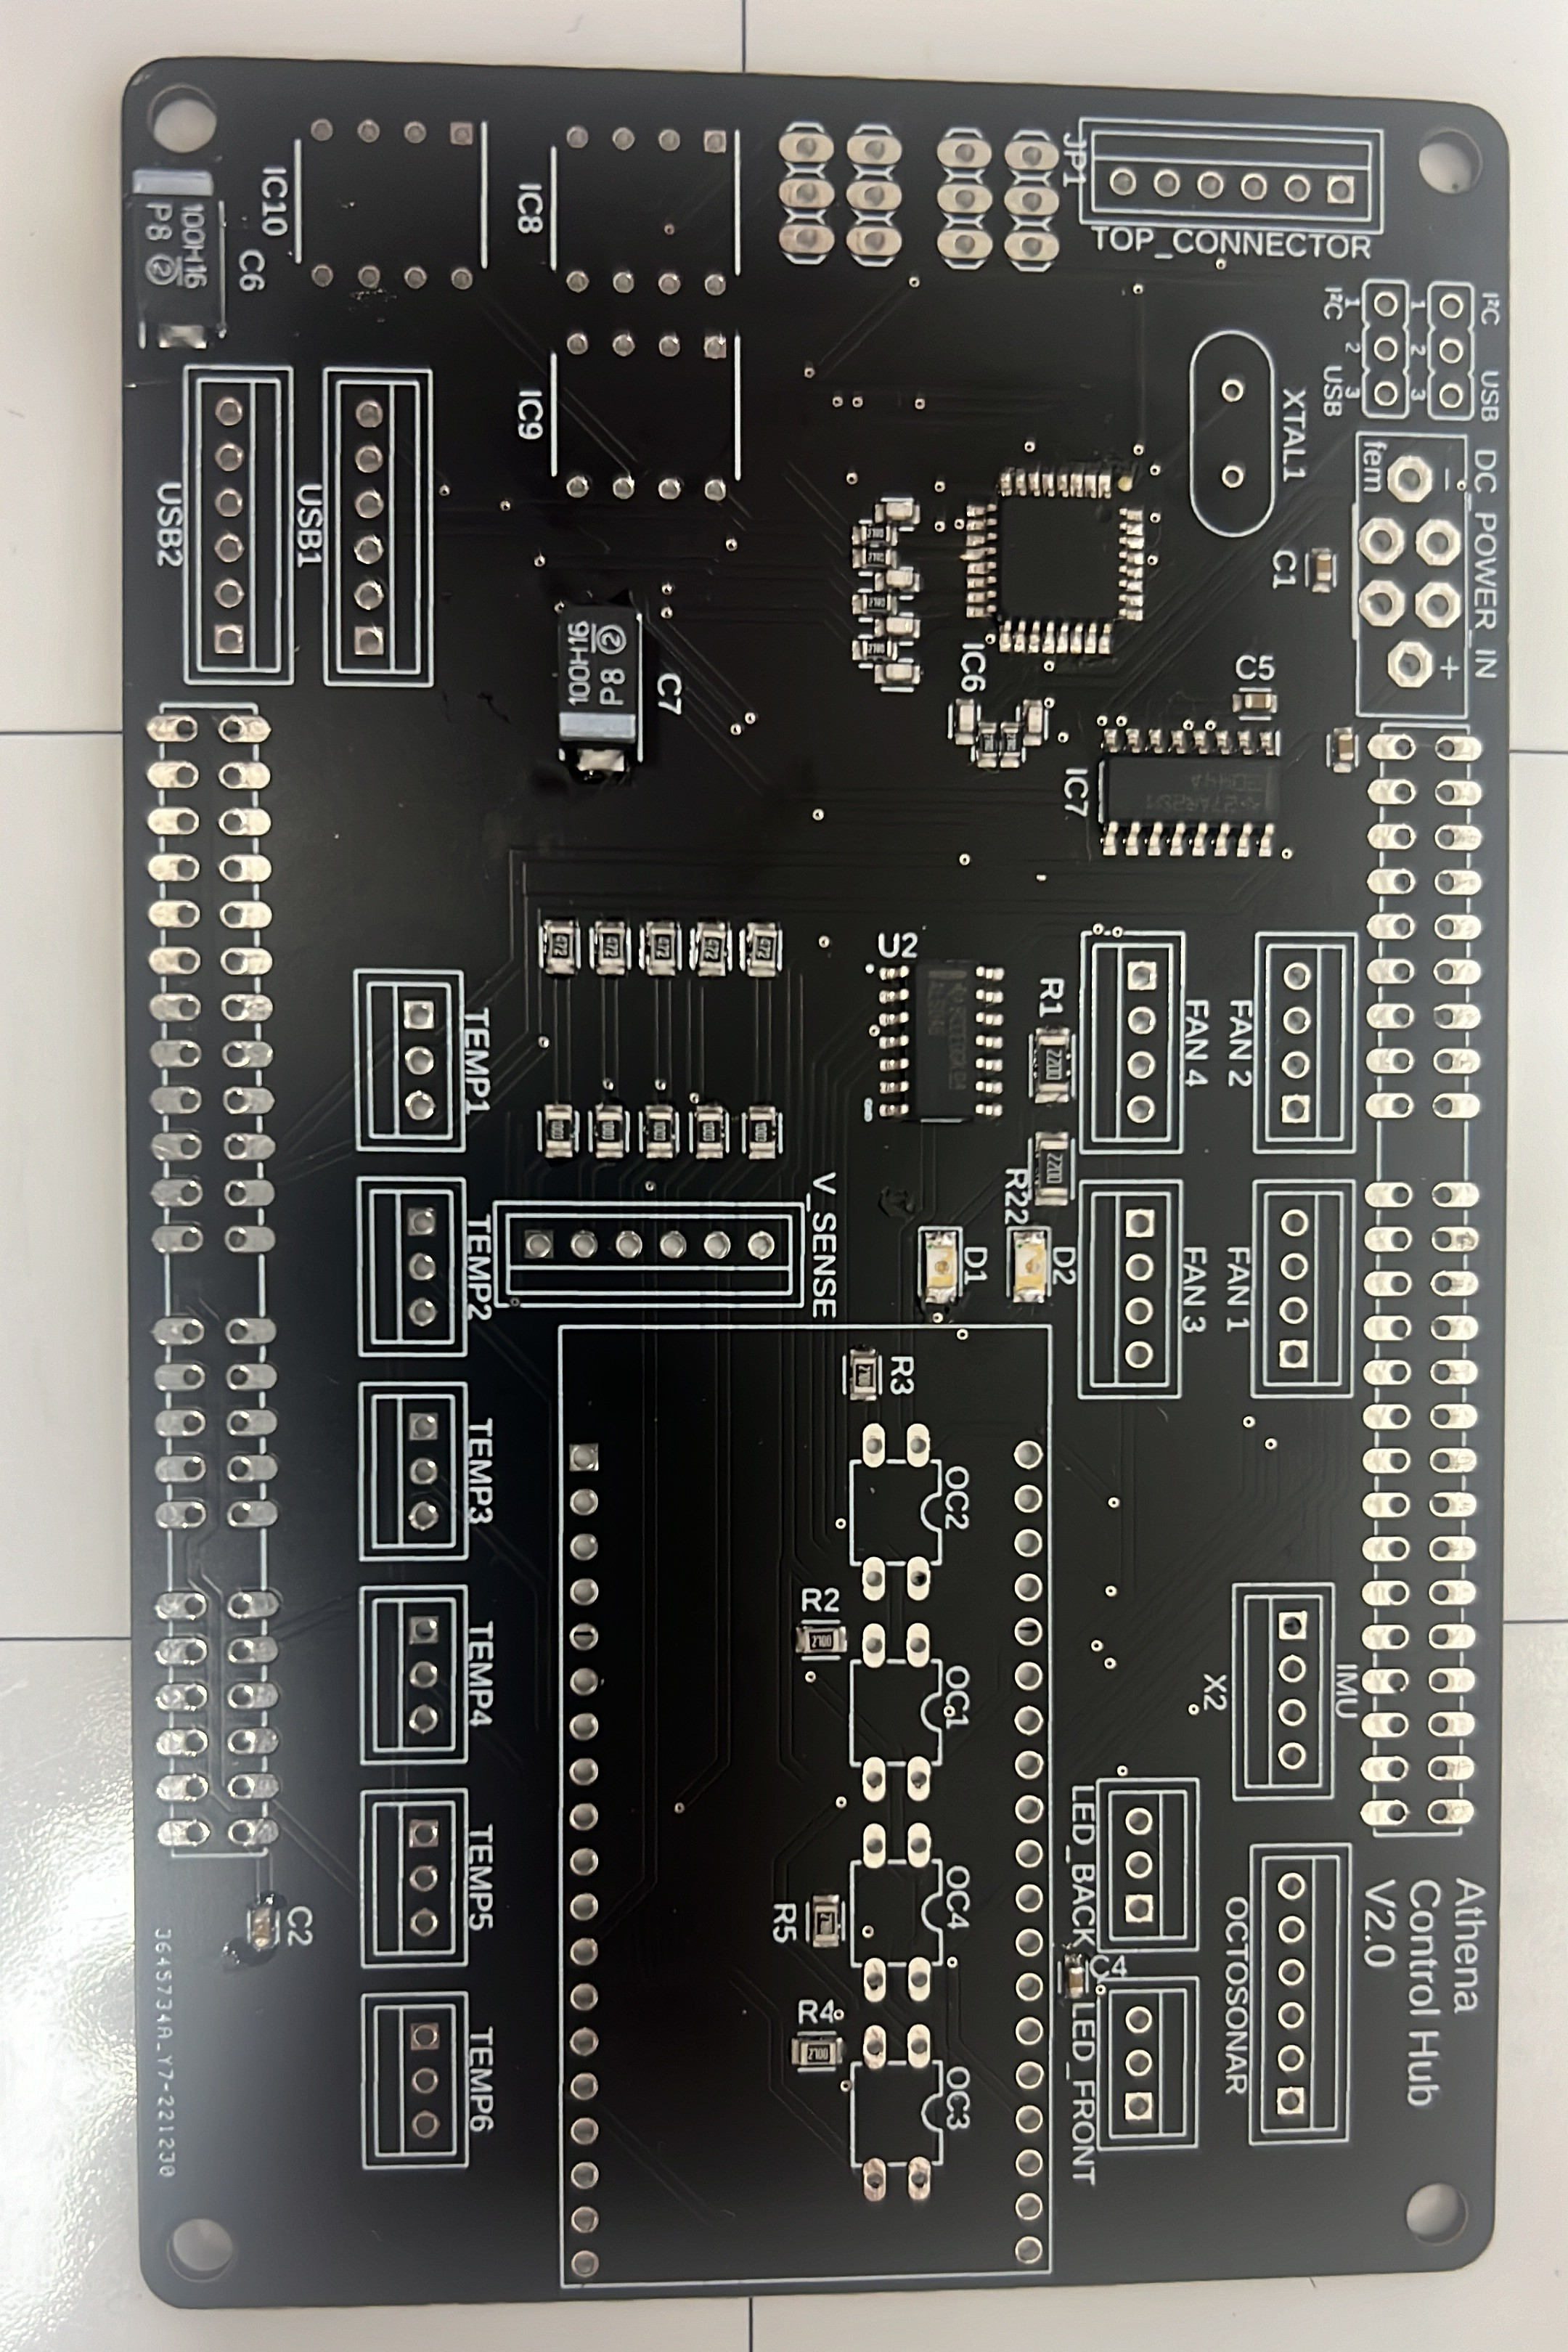
\includegraphics[scale=0.09]{./3_Stand_der_Technik/Abbildungen/shield_done.jpg}}
        \caption{Symbolfoto, fertig verl�tete Platine f�r den Bordcomputer.}
    \end{minipage}
\end{figure}

